\documentclass{article}

\usepackage[T1]{fontenc}
\usepackage{microtype}
\usepackage{graphicx}
\usepackage{subcaption}
\usepackage{booktabs}
\usepackage{hyperref}
\newcommand{\theHalgorithm}{\arabic{algorithm}}
\usepackage{icml2026}

\usepackage{amsmath}
\usepackage{amssymb}
\usepackage{mathtools}
\usepackage{amsthm}
\usepackage[capitalize,noabbrev]{cleveref}
\usepackage{xcolor}
\usepackage[textsize=tiny]{todonotes}

\theoremstyle{plain}
\newtheorem{theorem}{Theorem}[section]
\newtheorem{proposition}[theorem]{Proposition}
\newtheorem{lemma}[theorem]{Lemma}
\newtheorem{corollary}[theorem]{Corollary}
\theoremstyle{definition}
\newtheorem{definition}[theorem]{Definition}
\theoremstyle{remark}
\newtheorem{remark}[theorem]{Remark}

% Findings are the paper's unit of evidence: one claim, its number, and the table or
% figure that supports it.
\newcounter{finding}
\crefname{finding}{Finding}{Findings}
\usepackage{framed}
\renewenvironment{leftbar}{\def\FrameCommand{{\color{black!70}\vrule width 1.5pt}\hspace{5pt}}\MakeFramed{\advance\hsize-\width\FrameRestore}}{\endMakeFramed}
\newcommand{\finding}[2]{\begin{leftbar}\refstepcounter{finding}\label{#1}\noindent\textbf{Finding \thefinding.} #2\end{leftbar}}
\newcommand{\taueff}{\tau_{\mathrm{eff}}}
\newcommand{\Aref}{A_{1}}
\newcommand{\Atau}{A_{\tau}}
\newcommand{\At}[1]{A_{#1}}
\newcommand{\Spr}{\operatorname{Spr}}
\newcommand{\E}{\mathbb{E}}
\newcommand{\TODO}[1]{\todo[inline,color=orange!25]{TODO: #1}}

% Every number quoted in the text comes from this generated file (src/cavla/paper_numbers.py).
% Generated by src/cavla/paper_numbers.py; do not edit by hand.
\newcommand{\NClips}{60}
\newcommand{\EOneSpreadMin}{9}
\newcommand{\EOneSpreadMax}{14}
\newcommand{\AOneFiveEFourTau}{0.64}
\newcommand{\AOneFiveEFourTauLo}{0.59}
\newcommand{\AOneFiveEFourTauHi}{0.67}
\newcommand{\AOneFiveEFourContraction}{0.68}
\newcommand{\AOneFiveEFourFracContracted}{92}
\newcommand{\AOneFiveEFourExplAde}{97}
\newcommand{\AOneFiveEFourExplFlip}{86}
\newcommand{\AOneFiveETenTau}{0.83}
\newcommand{\AOneFiveETenTauLo}{0.80}
\newcommand{\AOneFiveETenTauHi}{0.86}
\newcommand{\AOneFiveETenContraction}{0.86}
\newcommand{\AOneFiveETenFracContracted}{90}
\newcommand{\AOneFiveETenExplAde}{121}
\newcommand{\AOneFiveETenExplFlip}{90}
\newcommand{\AOneFiveHeunThreeFlipResid}{16.5}
\newcommand{\AOneFiveHeunFiveFlipResid}{9.1}
\newcommand{\AOneFiveStopsRef}{6}
\newcommand{\AOneFiveStopsEFour}{5}
\newcommand{\AOneFiveStopsLow}{7}
\newcommand{\ROneEFourTau}{0.61}
\newcommand{\ROneEFourTauLo}{0.59}
\newcommand{\ROneEFourTauHi}{0.63}
\newcommand{\ROneEFourContraction}{0.66}
\newcommand{\ROneEFourFracContracted}{93}
\newcommand{\ROneEFourExplAde}{86}
\newcommand{\ROneEFourExplFlip}{119}
\newcommand{\ROneETenTau}{0.84}
\newcommand{\ROneETenTauLo}{0.82}
\newcommand{\ROneETenTauHi}{0.85}
\newcommand{\ROneETenContraction}{0.84}
\newcommand{\ROneETenFracContracted}{93}
\newcommand{\ROneETenExplAde}{92}
\newcommand{\ROneETenExplFlip}{100}
\newcommand{\ROneStopsRef}{6}
\newcommand{\ROneStopsEFour}{4}
\newcommand{\ROneStopsLow}{8}
\newcommand{\ATwoEFourTau}{0.62}
\newcommand{\ATwoEFourTauLo}{0.55}
\newcommand{\ATwoEFourTauHi}{0.67}
\newcommand{\ATwoEFourContraction}{0.67}
\newcommand{\ATwoEFourFracContracted}{92}
\newcommand{\ATwoEFourExplAde}{114}
\newcommand{\ATwoEFourExplFlip}{90}
\newcommand{\ATwoETenTau}{0.83}
\newcommand{\ATwoETenTauLo}{0.81}
\newcommand{\ATwoETenTauHi}{0.85}
\newcommand{\ATwoETenContraction}{0.85}
\newcommand{\ATwoETenFracContracted}{90}
\newcommand{\ATwoETenExplAde}{115}
\newcommand{\ATwoETenExplFlip}{79}
\newcommand{\ATwoStopsRef}{6}
\newcommand{\ATwoStopsEFour}{4}
\newcommand{\ATwoStopsLow}{9}
\newcommand{\StopClips}{4}
\newcommand{\StopPlans}{360}

% Generated by paper/tables/make_tables.py; do not edit by hand.
\newcommand{\AOneFiveHeunThreeTau}{0.95}
\newcommand{\AOneFiveHeunThreeFlip}{17.8}
\newcommand{\AOneFiveHeunThreeFlipMatched}{1.3}
\newcommand{\AOneFiveHeunFiveTau}{0.98}
\newcommand{\AOneFiveHeunFiveFlip}{9.7}
\newcommand{\AOneFiveHeunFiveFlipMatched}{0.6}
\newcommand{\GaussEFour}{0.67}
\newcommand{\GaussETen}{0.86}
\newcommand{\ExplMin}{79}
\newcommand{\ExplMax}{121}
\newcommand{\ExplRatioMin}{0.79}
\newcommand{\ExplRatioMax}{1.21}
\newcommand{\FlipResidMaxAbs}{2.04}
\newcommand{\MinadeResidMin}{0.00}
\newcommand{\MinadeResidMax}{0.11}
\newcommand{\MinadeResidPos}{5}
\newcommand{\NCells}{6}
\newcommand{\EntropyResidMin}{-0.03}
\newcommand{\EntropyResidMax}{0.03}
\newcommand{\EOneFlipResidMin}{11}
\newcommand{\EOneFlipResidMax}{15}
\newcommand{\ATwoETenFlipResid}{2.0}
\newcommand{\ATwoETenFlipResidLo}{0.03}
\newcommand{\ATwoETenFlipResidHi}{4.4}
\newcommand{\SigEulerFour}{0.66--0.68}
\newcommand{\SigTempFour}{0.69--0.73}
\newcommand{\SigShrinkFour}{0.53--0.55}
\newcommand{\SigEulerTen}{0.84--0.86}
\newcommand{\SigTempTen}{0.84--0.87}
\newcommand{\SigShrinkTen}{0.78}
\newcommand{\SigEulerFrac}{90--93}
\newcommand{\SigTempFrac}{81--89}
\newcommand{\StopClipMaxSpeed}{2.6}
\newcommand{\SigDiffTempFour}{$-$0.037\,[$-$0.071,\,$-$0.012]}
\newcommand{\SigDiffShrinkFour}{0.128\,[0.108,\,0.147]}
\newcommand{\SigDiffFracFour}{7.1\,[4.4,\,9.9]}
\newcommand{\SigDiffTempTen}{$-$0.002\,[$-$0.020,\,0.014]}
\newcommand{\SigDiffShrinkTen}{0.067\,[0.056,\,0.076]}
\newcommand{\SigDiffFracTen}{4.8\,[1.8,\,7.8]}
\newcommand{\ShrinkFlipResidMin}{0.7}
\newcommand{\ShrinkFlipResidMax}{3.4}
\newcommand{\ShrinkContrFour}{0.53--0.55}
\newcommand{\ShrinkContrTen}{0.78}
\newcommand{\FDClips}{60}
\newcommand{\FDTau}{0.64}
\newcommand{\FDGain}{0.28}
\newcommand{\FDTauCI}{[0.63,\,0.65]}
\newcommand{\FDResidHi}{0.051}
\newcommand{\FDGainEEight}{0.12}
\newcommand{\FDVsEFour}{$-$0.001\,[$-$0.033,\,0.032]}
\newcommand{\FDGainEEightCI}{[0.09,\,0.14]}
\newcommand{\FDEEightResid}{0.016\,[$-$0.014,\,0.048]}
\newcommand{\FDResidPt}{0.008}
\newcommand{\FDEFourTau}{0.63}
\newcommand{\FDEFourResidHi}{0.070}
\newcommand{\FDResid}{0.008\,[$-$0.034,\,0.051]}
\newcommand{\FDETenTau}{0.84}
\newcommand{\FDETenResid}{0.012\,[$-$0.016,\,0.041]}
\newcommand{\NClipsInTrain}{57}
\newcommand{\QDClips}{60}
\newcommand{\QDConvMM}{1.5}
\newcommand{\QDRefSpread}{0.14}
\newcommand{\QDRefADE}{1.55}
\newcommand{\QDETenTau}{0.98}
\newcommand{\QDETenResid}{0.001\,[0.000,\,0.001]}
\newcommand{\QDEFourTau}{0.42\,[0.41,\,0.44]}
\newcommand{\QDEFourResid}{0.041\,[0.022,\,0.062]}
\newcommand{\QDEFourMatchedGain}{0.001}
\newcommand{\QDEFourFlipResid}{2.6\,[$-$1.4,\,7.2]}
\newcommand{\QDSftEFourTau}{0.37\,[0.36,\,0.39]}
\newcommand{\QDSftEFourResid}{0.018\,[$-$0.002,\,0.039]}
\newcommand{\QDSftEFourFlipResid}{3.5\,[0.0,\,7.5]}
\newcommand{\QDSftEFourMatchedGain}{0.002}
\newcommand{\QDEFourFlip}{4.4}
\newcommand{\QDEFourFlipMatched}{1.8}


\icmltitlerunning{When Fewer Steps Mean Lower Temperature}

\begin{document}

\twocolumn[
  \icmltitle{When Fewer Steps Mean Lower Temperature:\texorpdfstring{\\}{ }
    Euler Sampling of Flow-Matching Driving Policies}

  \icmlsetsymbol{equal}{*}
  \begin{icmlauthorlist}
    \icmlauthor{Anonymous Authors}{anon}
  \end{icmlauthorlist}
  \icmlaffiliation{anon}{Anonymous Institution}
  \icmlcorrespondingauthor{Anonymous Authors}{anon@anon.edu}
  \icmlkeywords{flow matching, vision-language-action models, autonomous driving, ODE solvers, sampling temperature}
  \vskip 0.3in
]

\printAffiliationsAndNotice{}

\begin{abstract}
Flow-matching driving policies are made faster by integrating with fewer Euler steps, and the change is usually reported as preserving or improving accuracy. We show that few-step Euler samplers contract their samples toward the conditional mean, and that an accurate reference solver run at a lower sampling temperature reproduces what this contraction does to the metrics used to evaluate them. One Euler step returns the conditional mean, and more steps contract samples toward it by an amount that a closed-form Gaussian factor matches at the median. On \NClips{} clips from the PhysicalAI-AV test split, the released 10-step samplers of three Alpamayo generations share an effective temperature of \AOneFiveETenTau--\ROneETenTau. At that temperature the reference solver reproduces their change in single-sample error and in the share of changed driving decisions (flip-rate residuals at most \FlipResidMaxAbs{} points, although only R1's $E_{10}$ passes our equivalence test on both metrics), whereas second-order Heun samplers with a similar budget change \AOneFiveHeunFiveFlipResid--\AOneFiveHeunThreeFlipResid{} points more decisions than their matched temperature. On the original Alpamayo-1.5 checkpoint and the same clips, a published velocity cache (FlashDrive) lowers single-sample error by \FDGainEEight\,m relative to plain 8-step Euler and behaves like four Euler steps ($\taueff$ \FDTau); its error residual against the reference at that temperature is \FDResidPt\,m, close to but not within our equivalence margin. The match holds for rates over clips, not for the same noise, and a linear shrinkage toward the mean passes it too. We therefore propose that accuracy gains from fewer steps be reported against a reference solver at matched effective temperature, and we give a protocol and its statistics for doing so.
\end{abstract}

% ---------------------------------------------------------------------------
\section{Introduction}
\label{sec:intro}

Integrating Alpamayo-1.5 with four Euler steps instead of the released ten lowers its single-sample error against the human trajectory and changes about one decision in ten, compared with an accurate reference solver (\cref{fig:teaser,tab:matched}). Should the improvement be credited to the faster sampler? We argue that it should not: the same improvement, and nearly the same decision changes, are obtained by keeping the reference solver and shrinking the initial noise.

The reason is elementary. Under rectified-flow interpolation~\citep{lipman2023flow,liu2023rectified} the initial velocity is $v(z,0)=\E[x_1\mid c]-z$, so a single Euler step returns the conditional mean, and more steps move toward the exact flow. A $k$-step Euler sampler therefore sits between the mean and the policy's distribution, the same place a lower sampling temperature puts it. Accelerations that build on first-order integration~\citep{flashdrive2026,probeflow2026,adavla2026,coda2026} can inherit this temperature shift; we test one of them, FlashDrive's velocity cache (\cref{find:flash}). Single-sample metrics such as ADE$_1$ register it as an accuracy gain, while best-of-$k$ metrics such as minADE$_6$ get worse.

\begin{figure}[t]
  \centering
  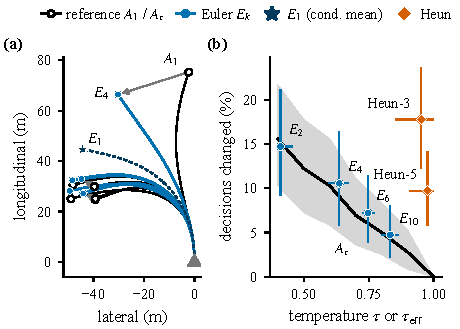
\includegraphics[width=\linewidth]{figures/fig_teaser.pdf}
  \caption{\textbf{Fewer Euler steps behave like a lower temperature; Heun steps do not.}
  (a)~One PhysicalAI-AV test clip (Alpamayo-1.5, ego at 10.5\,m/s), bird's-eye view, six shared noises.
  Four Euler steps ($E_4$, blue) move every sample of the reference solver ($\Aref$, black) toward the
  one-step conditional mean ($E_1$, star); the one seed that goes straight under $\Aref$ turns left.
  (b)~Share of decisions that differ from $\Aref$ under the same noise. Black: the reference solver started
  from $\tau z$ (95\% clip-bootstrap band). Euler samplers placed at their effective temperature fall on the
  curve; Heun-3 and Heun-5 change \AOneFiveHeunThreeFlip\% and \AOneFiveHeunFiveFlip\% of decisions at almost no change in temperature.
  \NClips{} clips $\times$ 6 seeds; bars are 95\% intervals.}
  \label{fig:teaser}
\end{figure}

\paragraph{Contributions.}
\begin{itemize}
  \item \textbf{A matched-temperature evaluation protocol} for accelerated flow samplers: estimate the sampler's effective temperature $\taueff$ from its seed spread, compare it with the reference solver run at $\taueff$, and report effect, residual and equivalence with clip-level intervals (\cref{sec:protocol}).
  \item \textbf{Evidence on three generations of a production driving VLA} on PhysicalAI-AV driving logs. The released samplers share $\taueff\approx0.83$; lowering the temperature alone changes ADE$_1$ and flip rate by \ExplRatioMin--\ExplRatioMax{} times what $E_4$ and $E_{10}$ change them; Heun-3 and Heun-5 fail the same test (\cref{fig:curves,tab:matched}); FlashDrive's velocity cache acts as a lower temperature (\cref{find:flash}).
  \item \textbf{A mechanism with a closed form.} Contraction toward the conditional mean (\cref{fig:mechanism}), the Gaussian factor $\prod_i\cos\theta_i$ that matches it at the median, and a symmetry condition under which no integrator changes a decision (\cref{sec:theory}).
  \item \textbf{A second family.} On Qwen-Drive, whose seed spread is a tenth of its error, step count still maps to temperature, but temperature does not change its error, so fewer steps only cost accuracy (\cref{sec:discussion}).
\end{itemize}
\TODO{Add the AlpaSim closed-loop contribution when the run finishes; keep only what the data support.}

% ---------------------------------------------------------------------------
\section{Background and Notation}
\label{sec:background}

\paragraph{Flow-matching driving policies.} A VLA driving policy encodes cameras, ego history and a reasoning trace into a context $c$ and decodes an action $x_1$ (64 normalized acceleration and curvature commands over 6.4\,s in Alpamayo) by integrating $v_\theta(x,t\mid c)$ from $x_0=z\sim\mathcal{N}(0,I)$ to $t=1$. With $x_t=(1-t)z+tx_1$, the flow-matching minimizer is $v(x,t)=\E[x_1-z\mid x_t=x,c]$. The released policies use forward Euler with 10 uniform steps~\citep{alpamayo2025}.

\paragraph{Notation.} $E_k$ is Euler with $k$ uniform steps; Heun-$k$ uses $2k$ field evaluations. $\Atau$ is the reference solver, Heun with 32 steps (64 evaluations), started from $\tau z$; $\Aref$ is the reference at $\tau=1$. All samplers for a clip share the same context, reasoning trace and six noises. $\Spr(S)$ is the mean pairwise distance between the trajectories $S$ produces from different noises. A \emph{flip} is a change of decision class relative to $\Aref$ under the same noise. ADE$_1$ is the mean single-sample displacement to the logged human trajectory.

\paragraph{Accelerations.} FlashDrive reuses the velocity on the 4th to 7th of 8 Euler steps~\citep{flashdrive2026}; ProbeFlow and AdaVLA adapt the number of steps~\citep{probeflow2026,adavla2026}; entropic time places steps by information about the output~\citep{stancevic2025entropic}; Coda corrects a few-step endpoint~\citep{coda2026}.

% ---------------------------------------------------------------------------
\section{Why Euler Steps Act Like Temperature}
\label{sec:theory}

\paragraph{One Euler step returns the conditional mean.} Since $x_0=z$, $E_1(z)=z+v(z,0)=\E[x_1\mid c]$ for every $z$: with the exact field the one-step sampler has no diversity at all. Learned fields are not exact, and $E_1$ keeps \EOneSpreadMin--\EOneSpreadMax\% of the reference solver's seed spread in our models.

\paragraph{Gaussian targets: contraction on any grid.} For $p(x_1\mid c)=\mathcal{N}(m,\operatorname{diag}(s^2))$ the field is linear and coordinate $d$ evolves with scale $\|u_d(t)\|$, where $u_d(t)=(1-t,\,ts_d)$. One Euler step from $t_i$ to $t_{i+1}$ multiplies coordinate $d$'s deviation from $m_d$ by $\langle u_d(t_i),u_d(t_{i+1})\rangle/\|u_d(t_i)\|^2$, whereas the exact flow multiplies it by $\|u_d(t_{i+1})\|/\|u_d(t_i)\|$. Writing $\theta_{d,i}$ for the angle between $u_d(t_i)$ and $u_d(t_{i+1})$,
\begin{equation}
  \frac{E_k(z)_d-m_d}{\Aref(z)_d-m_d}=\prod_{i=0}^{k-1}\cos\theta_{d,i}\;\le\;1
  \label{eq:contraction}
\end{equation}
on any grid (\cref{fig:mechanism}a). The inequality is implicit in the proof of Proposition~2 of~\citet{claustre2026gaussian}; we use the closed form as a prediction. The factor is symmetric in $s_d$ and $1/s_d$; for $0.3\le s_d\le3.3$ the factor of $E_{10}$ lies between 0.82 and 0.88. The angles $\theta_{d,i}$ sum to $\pi/2$, the angle between $u_d(0)$ and $u_d(1)$, and $\log\cos$ is concave, so on any grid the factor is at most $\cos(\pi/2k)^k$, with equality when all angles are equal: 0.883 for $E_{10}$, 0.729 for $E_4$ and 0.5 for $E_2$. Choosing where the steps go can reduce the contraction toward this cap but cannot remove it. Coordinates outside this range contract more but carry little of the spread, so the aggregate factor is set by the high-variance coordinates.

\begin{figure}[t]
  \centering
  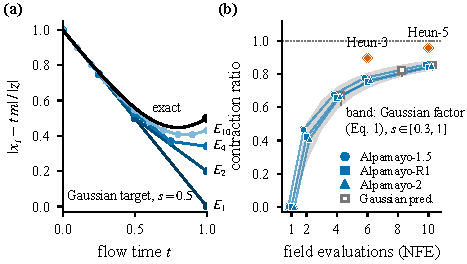
\includegraphics[width=\linewidth]{figures/fig_mechanism.pdf}
  \caption{\textbf{Euler contracts samples toward the conditional mean by the Gaussian factor of \cref{eq:contraction}.}
  (a)~One coordinate of a Gaussian target ($s=0.5$): deviation from the mean path under the exact flow (black)
  and under $k$ Euler steps (blue, darker $=$ fewer steps). Each step loses a factor $\cos\theta_i$, so $E_k$ ends
  at 0, 0.40, 0.68 and 0.86 of the exact deviation for $k=1,2,4,10$.
  (b)~Median ratio of each sample's distance to $E_1$ over the reference sample's, same noise, against field
  evaluations (NFE); three Alpamayo generations, \NClips{} clips $\times$ 6 seeds. Band: the Gaussian factor for
  $s\in[0.3,1]$; squares: its prediction from Alpamayo-1.5's conditional action variance (median and IQR;
  a separate sample of 200 clips, action space). Heun samplers (vermillion) barely contract at the same budget.}
  \label{fig:mechanism}
\end{figure}

\paragraph{Decisions protected by symmetry do not flip.}
\begin{proposition}
\label{prop:symmetry}
Let $g$ be an orthogonal reflection with fixed hyperplane $H$, let $p(x_1\mid c)$ be $g$-invariant, and let the decision be the side of $H$. An explicit Runge--Kutta integrator whose steps satisfy $h\,\mathrm{Lip}(v(\cdot,t))<1$ returns the decision of the exact flow for almost every $z$.
\end{proposition}
\noindent The field is $g$-equivariant and hence tangent to $H$ on $H$; each step is an equivariant homeomorphism mapping $H$ to itself and depending continuously on $h$, so half-spaces are preserved. Decision flips therefore need an asymmetric context. \TODO{full proof in the appendix; the Lipschitz condition can fail near $t=1$, discuss.}

% ---------------------------------------------------------------------------
\section{Matched-Temperature Protocol and Setup}
\label{sec:protocol}
\begin{definition}
The effective temperature of a sampler $S$ is the $\tau$ at which $\Spr(\Atau)=\Spr(S)$, interpolated over $\tau\in\{1,0.9,\dots,0.4\}$.
\end{definition}
For a metric $M$ we report $M(\Aref)$, $M(S)$ and $M(A_{\taueff(S)})$. The \emph{residual} $M(S)-M(A_{\taueff(S)})$ is the part of the sampler's effect that temperature does not explain, and $1-\text{residual}/\text{effect}$ is the fraction explained. Clips are the independent unit: every quantity, including $\taueff$, is recomputed in each of 1000 bootstrap resamples of clips, drawn jointly across models because all models see the same clips. We call $S$ \emph{equivalent} to $\At{\taueff}$ on a metric when the 90\% interval of the residual lies inside a margin (two one-sided tests; 2 points for flip rates, 0.05\,m for ADE$_1$). We chose the margins after seeing the \NClips{} clips reported here; they are fixed for the confirmation sample. Fractions explained above 100\% mean that the explicit temperature overshoots the sampler's effect; we therefore read residuals and their intervals, not fractions, as evidence. The protocol compares distributions: the same noise can still produce different decisions under $S$ and $\At{\taueff}$ (\cref{sec:discussion}).

\paragraph{Budgets.} The reference solver uses 64 field evaluations (NFE). $E_k$ uses $k$; Heun-3 uses 6 and Heun-5 uses 10, so Heun-5 has the released sampler's budget and Heun-3 sits between $E_4$ and $E_{10}$.

\paragraph{Policies.} Alpamayo-1.5, Alpamayo-R1 and Alpamayo-2-Super, frozen. Our integrators run inside each model's own sampling call with the model's step function, so the reasoning trace is shared across samplers within a clip.
\paragraph{Data.} The same \NClips{} clips from the default test split of PhysicalAI-AV~\citep{physicalai2025} for every model (one clip per dataset chunk), six noise seeds each, with the current frame at 5.1\,s. This split is not the held-out split of the Alpamayo release (\texttt{alpamayo\_aligned}): \NClipsInTrain{} of the \NClips{} clips are in its training partition. Because every comparison is within one model on the same inputs, training exposure affects both sides of each comparison, but it may change how much error a lower temperature removes; a pre-registered replication on clips from the held-out partition is running. \TODO{held-out replication.}
\paragraph{Decisions.} Longitudinal (stop, decelerate, keep, accelerate) and lateral (left, right, lane shift, straight) classes are read from each plan with thresholds fixed in advance (\cref{app:protocols}).

% ---------------------------------------------------------------------------
\section{Results}
\label{sec:results}

\begin{figure*}[t]
  \centering
  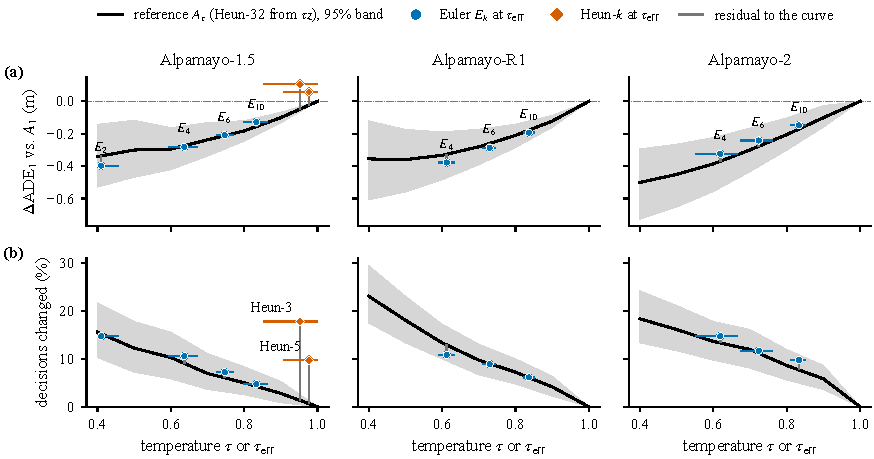
\includegraphics{figures/fig_curves_2row.pdf}
  \caption{\textbf{Placed at its effective temperature, each Euler sampler lands on the explicit-temperature curve; Heun samplers do not.}
  Black: the reference solver started from $\tau z$, as a change from $\tau{=}1$, with a 95\% clip-bootstrap band.
  Blue: Euler with $k$ steps at its effective temperature (\cref{sec:protocol}; horizontal bars are 95\% intervals);
  vermillion: Heun-3 and Heun-5. Gray ticks join each sampler to the curve at the same $\tau$; their length is the
  residual of \cref{tab:matched}. (a)~Single-sample error falls with temperature, and Euler follows it.
  (b)~Euler changes about as many decisions as the reference at the same temperature; Heun changes 10--18\% of decisions
  at $\taueff\approx1$. $E_1$, and $E_2$ for Alpamayo-R1 and -2, have $\taueff<0.4$ and are not shown.
  \NClips{} PhysicalAI-AV clips (default test split) $\times$ 6 seeds per model. Best-of-six error is in \cref{app:extra}.}
  \label{fig:curves}
\end{figure*}

\finding{find:contraction}{\emph{Euler samples contract toward the conditional mean; Heun samples do not.} In trajectory space, \AOneFiveEFourFracContracted--\ROneEFourFracContracted\% of $E_4$ and \AOneFiveETenFracContracted--\ROneETenFracContracted\% of $E_{10}$ samples lie closer to the one-step mean than the reference sample from the same noise, with median ratios \ROneEFourContraction--\AOneFiveEFourContraction{} for $E_4$ and \ROneETenContraction--\AOneFiveETenContraction{} for $E_{10}$ across the three models. The Gaussian factor of \cref{eq:contraction}, computed from Alpamayo-1.5's conditional action variance, gives \GaussEFour{} and \GaussETen{} (\cref{fig:mechanism}; per-model values in \cref{tab:contraction}). It matches the median but not the ranking of clips, so we use it as an explanation of the typical value rather than as a per-clip predictor.}

\begin{table*}[t]
  \caption{\textbf{Euler samplers land on the explicit-temperature curve; Heun samplers do not.} For each sampler $S$ we report the reference solver at $\tau{=}1$ ($\Aref$), the sampler, and the reference solver at the sampler's effective temperature ($A_{\taueff}$). Flips are decision changes relative to $\Aref$ under the same noise; the last column is the flip residual $S-A_{\taueff}$ with a 95\% interval from a bootstrap over clips. Shrink$_k$ is a control with no integrator: each $\Aref$ sample moved linearly toward $E_1$ to $E_k$'s spread. 60 PhysicalAI-AV test clips $\times$ 6 seeds per model.}
  \label{tab:matched}
  \centering\small\setlength{\tabcolsep}{5pt}
  \begin{tabular}{@{}llccccccc@{}}
    \toprule
    & & & \multicolumn{3}{c}{ADE$_1$ (m)} & \multicolumn{3}{c}{Decision flips (\%)} \\
    \cmidrule(lr){4-6}\cmidrule(l){7-9}
    Model & Sampler $S$ & $\taueff$ & $\Aref$ & $S$ & $A_{\taueff}$ & $S$ & $A_{\taueff}$ & $S-A_{\taueff}$ \\
    \midrule
    Alpamayo-1.5 & $E_4$ & 0.64 & 2.86 & 2.58 & 2.58 & 10.6 & 9.1 & 1.5\,{\scriptsize[$-$1.3,\,5.3]} \\
     & Shrink$_4$ & 0.64 & 2.86 & 2.53 & 2.58 & 10.0 & 9.1 & 0.9\,{\scriptsize[$-$2.9,\,4.8]} \\
     & $E_{10}$ & 0.83 & 2.86 & 2.73 & 2.70 & 4.7 & 4.3 & 0.5\,{\scriptsize[$-$1.2,\,2.3]} \\
     & Shrink$_{10}$ & 0.83 & 2.86 & 2.68 & 2.70 & 5.0 & 4.3 & 0.7\,{\scriptsize[$-$1.1,\,2.9]} \\
     & Heun-3 & 0.95 & 2.86 & 2.96 & 2.81 & 17.8 & 1.3 & 16.5\,{\scriptsize[9.8,\,23.1]} \\
     & Heun-5 & 0.98 & 2.86 & 2.91 & 2.83 & 9.7 & 0.6 & 9.1\,{\scriptsize[4.3,\,14.2]} \\
    \midrule
    Alpamayo-R1 & $E_4$ & 0.61 & 2.47 & 2.10 & 2.15 & 10.8 & 12.9 & $-$2.0\,{\scriptsize[$-$5.7,\,1.2]} \\
     & Shrink$_4$ & 0.61 & 2.47 & 2.11 & 2.15 & 14.2 & 12.9 & 1.3\,{\scriptsize[$-$2.8,\,5.3]} \\
     & $E_{10}$ & 0.84 & 2.47 & 2.28 & 2.30 & 6.1 & 6.1 & 0.0\,{\scriptsize[$-$2.0,\,1.9]} \\
     & Shrink$_{10}$ & 0.84 & 2.47 & 2.28 & 2.30 & 7.8 & 6.1 & 1.7\,{\scriptsize[$-$0.5,\,4.0]} \\
    \midrule
    Alpamayo-2 & $E_4$ & 0.62 & 2.93 & 2.61 & 2.56 & 14.7 & 13.3 & 1.4\,{\scriptsize[$-$1.6,\,4.9]} \\
     & Shrink$_4$ & 0.62 & 2.93 & 2.60 & 2.56 & 16.7 & 13.3 & 3.4\,{\scriptsize[$-$0.5,\,7.9]} \\
     & $E_{10}$ & 0.83 & 2.93 & 2.78 & 2.76 & 9.7 & 7.7 & 2.0\,{\scriptsize[0.03,\,4.4]} \\
     & Shrink$_{10}$ & 0.83 & 2.93 & 2.75 & 2.76 & 8.3 & 7.7 & 0.7\,{\scriptsize[$-$2.1,\,3.3]} \\
    \bottomrule
  \end{tabular}
\end{table*}


\finding{find:matched}{\emph{The released samplers share one effective temperature, and temperature accounts for most of what they change.} $\taueff(E_{10})$ is \AOneFiveETenTau{} [\AOneFiveETenTauLo, \AOneFiveETenTauHi], \ROneETenTau{} [\ROneETenTauLo, \ROneETenTauHi] and \ATwoETenTau{} [\ATwoETenTauLo, \ATwoETenTauHi] for the three generations. The reference solver at $\taueff$ changes ADE$_1$ and flip rate by \ExplRatioMin--\ExplRatioMax{} times what $E_4$ and $E_{10}$ change them (\cref{fig:curves,tab:matched}; above one, temperature moves it more). Flip residuals are at most \FlipResidMaxAbs{} points in absolute value. With \NClips{} clips their intervals are too wide to establish equivalence at the 2-point margin in most cells, and one interval excludes zero: Alpamayo-2's $E_{10}$ changes \ATwoETenFlipResid{} points more decisions than its matched temperature [\ATwoETenFlipResidLo, \ATwoETenFlipResidHi]. Euler is not temperature in every respect. Its best-of-six error (minADE$_6$) is worse than the reference's, as fewer distinct samples imply, and slightly worse than the matched temperature (residual \MinadeResidMin{} to \MinadeResidMax\,m, positive in \MinadeResidPos{} of \NCells{} cells; \cref{app:extra}); decision-entropy residuals lie between \EntropyResidMin{} and \EntropyResidMax. \TODO{pre-registered confirmation on fresh clips and seeds (the 436 clips of \cref{app:schedules} were already used), primary endpoint $E_{10}$ equivalence averaged over models.}}

\finding{find:heun}{\emph{Second-order samplers fail the same test.} Heun-3 and Heun-5 barely contract ($\taueff$ \AOneFiveHeunThreeTau{} and \AOneFiveHeunFiveTau{} for Alpamayo-1.5), yet they flip \AOneFiveHeunThreeFlip\% and \AOneFiveHeunFiveFlip\% of decisions, against \AOneFiveHeunThreeFlipMatched\% and \AOneFiveHeunFiveFlipMatched\% for the reference solver at the same temperature; their flip residuals are $+$\AOneFiveHeunThreeFlipResid{} and $+$\AOneFiveHeunFiveFlipResid{} points (\cref{fig:curves,tab:matched}). Heun-5 has the released sampler's budget. The test therefore discriminates: landing on the temperature curve is not a property of every cheap sampler. Part of Heun's residual is its own integration error rather than a departure from a distribution, and we do not claim that every non-Euler sampler fails.}
\TODO{Heun-3/5 on Alpamayo-R1 and -2; a Heun control matched in displacement from $\Aref$.}

\finding{find:shrink}{\emph{Rates do not distinguish Euler from a linear shrinkage toward the mean; per-sample contraction separates them only in part.} Shrink$_k$ scales every reference sample's deviation from $E_1$ by one factor per model, chosen so that its spread equals $E_k$'s (\cref{tab:matched}). Its flip residuals are \ShrinkFlipResidMin{} to \ShrinkFlipResidMax{} points, all positive and all with intervals that contain zero. Because the factor is shared, every shrinkage sample has the same contraction ratio by construction, whereas Euler's ratios vary across samples. Pooled over the three models, Euler's median ratio exceeds the shrinkage's by \SigDiffShrinkFour{} at $E_4$'s spread and \SigDiffShrinkTen{} at $E_{10}$'s, and differs from the reference solver's at $\taueff$ by \SigDiffTempFour{} and \SigDiffTempTen; Euler contracts \SigDiffFracFour{} and \SigDiffFracTen{} percentage points more samples than temperature. Euler is therefore closer to temperature than to a uniform shrinkage, but not identical to it (the difference is largest for Alpamayo-R1), and a matching median does not by itself identify temperature. This comparison uses the same \NClips{} clips and is exploratory.}

\finding{find:flash}{\emph{A published acceleration behaves like a lower temperature.} FlashDrive reuses the velocity on the 4th to 7th of 8 Euler steps~\citep{flashdrive2026}. We implemented this cache ourselves inside FlashDrive's inference code and ran it on the original Alpamayo-1.5 checkpoint, on the same \FDClips{} clips with inputs from 4 consecutive 10\,Hz frames per clip; $\taueff$ values therefore differ slightly from \cref{tab:matched}. Relative to plain 8-step Euler, the cache lowers ADE$_1$ by \FDGainEEight\,m \FDGainEEightCI. Its $\taueff$ is \FDTau{} \FDTauCI, close to $E_4$'s \FDEFourTau, and its ADE$_1$ differs from $E_4$'s by \FDVsEFour\,m. Against the reference at its $\taueff$ (interpolated linearly between grid temperatures), its ADE$_1$ residual is \FDResid\,m. The upper bound exceeds our 0.05\,m margin, so equivalence is not established; nor is it for $E_4$ (upper bound \FDEFourResidHi), while $E_8$ (\FDEEightResid) and $E_{10}$ (\FDETenResid) pass. All intervals are 90\%, from a clip bootstrap that re-estimates $\taueff$. We report ADE$_1$ only; decision flips for this run are pending. Our pre-registered guess of $\taueff$ 0.5--0.6 for the cache was too low.}


\paragraph{The one-step limit.} $E_1$ contracts beyond the measured temperature range ($\taueff<0.4$). At $\tau=0.4$ the reference still changes \EOneFlipResidMin--\EOneFlipResidMax{} points fewer decisions than $E_1$, so our data do not show that $E_1$ is matched by any temperature. \TODO{reference at $\tau\in\{0.3,0.2,0.1\}$.}

\paragraph{Rare decisions.} Stopping is too rare in this sample to test: across the three models, the reference stops in \AOneFiveStopsRef{}, \ROneStopsRef{} and \ATwoStopsRef{} of 360 plans, coming from \StopClips{} clips in which the vehicle moves at most \StopClipMaxSpeed\,m/s. We observe that lowering $\tau$ adds stops while fewer Euler steps remove them, and leave a test of this tail behavior to a sample enriched for stopping scenes. Log-replay collisions with logged agents are similarly rare (differences between samplers come from a handful of clips) and are not used as evidence.

\TODO{FlashDrive's optimized checkpoint (W4A8, DFlash, streaming) at matched temperature (running); minADE$_k$ crossover on the unified sample.}

% ---------------------------------------------------------------------------
\section{Related Work}
\label{sec:related}
\paragraph{Accelerating VLA sampling.} FlashDrive, ProbeFlow, AdaVLA and Coda reduce or correct flow sampling and report trajectory or success metrics~\citep{flashdrive2026,probeflow2026,adavla2026,coda2026}. Our protocol separates the part of such gains that a temperature change reproduces.
\paragraph{Discretization and diversity.} Few-step generators lose rare modes in image synthesis~\citep{subflow2026}, few-step error has been attributed to predicting only the mean of the velocity distribution~\citep{chen2025gmflow}, and Euler on Gaussian flows has been analyzed by \citet{claustre2026gaussian}. Lowering temperature by scaling the prior noise is standard in generative flows and GANs~\citep{kingma2018glow,brock2019biggan}, and sampler discretization has been studied systematically for diffusion models~\citep{karras2022edm}. In driving, multimodal planners such as DiffusionDrive are designed against mode collapse~\citep{liao2025diffusiondrive}. We study the consequence for driving decisions.
\paragraph{Critical windows and schedules.} Speciation and symmetry breaking in diffusion~\citep{biroli2024dynamical,raya2023ssb} and entropic time~\citep{stancevic2025entropic} motivate where steps should go. A schedule that targets decision information passed a pre-registered confirmation on 436 clips not used to design it, yet its gain disappeared at matched temperature (\cref{app:schedules}); this negative result motivated the protocol.

% ---------------------------------------------------------------------------
\section{Discussion and Limitations}
\label{sec:discussion}
\paragraph{Recommendations.} Report $\taueff$ for any first-order or cached sampler, and compare against the reference solver at that temperature before attributing accuracy gains to the sampler. If lower temperature is desired, set it explicitly so that it is visible and tunable.
\paragraph{Distribution, not trajectory.} Matching holds for rates averaged over clips. Under the same noise, $E_4$ and the reference solver at $\taueff$ still disagree on a sizable share of individual decisions, and per-clip rates differ, so the two are not interchangeable sample by sample or clip by clip.
\paragraph{What the test identifies.} Matching spread and comparing rates does not single out temperature: a linear shrinkage toward $E_1$ passes it too, and per-sample contraction places Euler closer to temperature than to that shrinkage but not on it (\cref{find:shrink}). Our claim is therefore at the level of rates: few-step Euler is a contraction toward the conditional mean whose effect on rate metrics an explicit temperature reproduces. The per-sample signature is a secondary endpoint of the pre-registered confirmation, with its statistic (the pooled difference in median contraction from temperature at $E_{10}$'s spread) and margin (0.05) fixed before it runs. Heun fails the rate test because it changes decisions without contracting.
\paragraph{A second family.} Qwen-Drive's planner predicts the clean trajectory, is trained only for flow times $t\le0.9$, and its released sampler ends on the endpoint predicted at $t=0.9$~\citep{qwendrive2026}. We therefore integrate its reference with Heun-32 on $[0,0.9]$ followed by the same final endpoint (Heun-64 differs by at most \QDConvMM\,mm), and run its RL and SFT planners in reasoning mode with the planning expert in float32 on the same \QDClips{} clips. Its seed spread is small, \QDRefSpread\,m for both against an ADE$_1$ of \QDRefADE\,m (RL). The released 10-step sampler sits at $\tau_{\text{eff}}=\QDETenTau$ for both planners with an ADE$_1$ residual of \QDETenResid\,m (RL), and $E_4$ at $\tau_{\text{eff}}=\QDEFourTau$ (RL) and \QDSftEFourTau{} (SFT): step count maps to temperature in this family too. The accuracy does not follow. Lowering this model's temperature to $E_4$'s changes ADE$_1$ by \QDEFourMatchedGain\,m (RL) and \QDSftEFourMatchedGain\,m (SFT), while $E_4$ is worse than the reference at its own temperature by \QDEFourResid\,m (RL) and \QDSftEFourResid\,m (SFT), and changes more decisions, by \QDEFourFlipResid{} and \QDSftEFourFlipResid{} points. We had predicted all residuals within our margins; the RL error residual and the SFT flip residual fail. When the error is set by the conditional mean rather than by seed spread, fewer steps have no temperature gain to offer and pay only their discretization cost. The bound below \cref{eq:contraction} does not apply here: it concerns Euler on $[0,1]$, whereas this sampler stops at $t=0.9$ and jumps to the predicted endpoint.
\paragraph{Limitations.} Decision classes are read from plans with fixed thresholds rather than from executed behavior; the reasoning trace is fixed within a clip; \NClips{} clips do not establish equivalence at tight margins; rare decisions are untested; the positive replication comes from one model family, and the one planner of a second family (Qwen-Drive) has an error that does not depend on temperature. \TODO{multi-seed language ablation; ReCogDrive and DiffusionDrive on NAVSIM.}

\section*{Impact Statement}
This work concerns how accelerated autonomous-driving policies are evaluated. Gains that come from a hidden temperature change can hide shifts in the decision distribution, and reporting effective temperature makes such shifts visible. We used public data and frozen public checkpoints; no vehicles were driven.

\bibliography{references}
\bibliographystyle{icml2026}

\newpage
\appendix
\onecolumn
\section{Additional Results}
\label{app:extra}
\begin{table}[t]
  \caption{\textbf{Euler samplers contract toward the conditional mean; Heun does not.} Median ratio of each sample's distance to the one-step mean $E_1$ over the reference sample's distance, from the same noise (share of samples with ratio $<1$ in parentheses), 60 clips $\times$ 6 seeds. Gaussian: the closed-form factor of \cref{eq:contraction} from Alpamayo-1.5's conditional action variance (median over a separate sample of 200 clips in action space; it does not predict the per-clip ranking).}
  \label{tab:contraction}
  \centering\footnotesize\setlength{\tabcolsep}{3pt}
  \begin{tabular}{@{}lcccc@{}}
    \toprule
    Sampler & Alpamayo-1.5 & Alpamayo-R1 & Alpamayo-2 & Gaussian \\
    \midrule
    $E_4$ & 0.68 (92\%) & 0.66 (93\%) & 0.67 (92\%) & 0.67 \\
    $E_{10}$ & 0.86 (90\%) & 0.84 (93\%) & 0.85 (90\%) & 0.86 \\
    Heun-5 & 0.96 (69\%) & -- & -- & -- \\
    \bottomrule
  \end{tabular}
\end{table}

\begin{figure}[h]
  \centering
  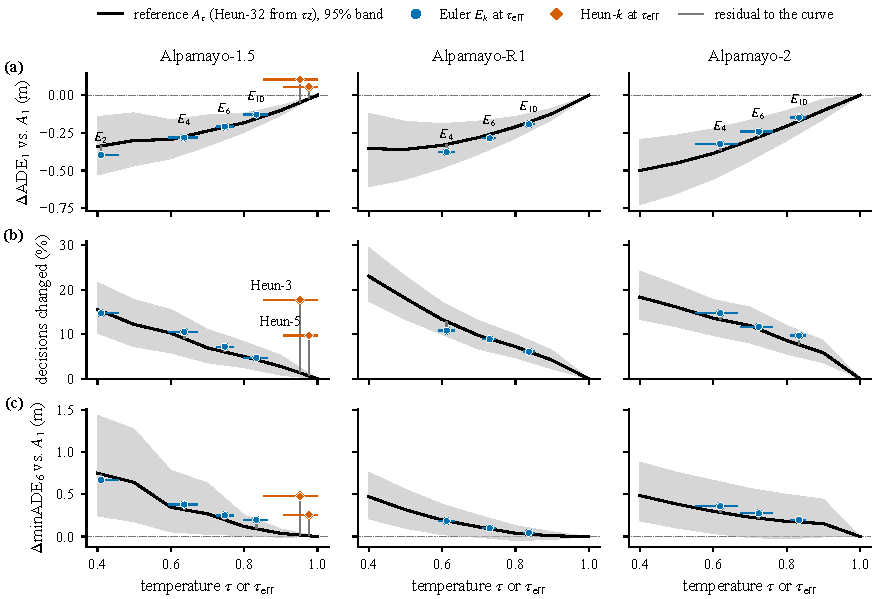
\includegraphics{figures/fig_curves.pdf}
  \caption{As \cref{fig:curves}, with (c) best-of-six error (minADE$_6$) as a change from $\Aref$. Euler lies slightly above the temperature curve: fewer distinct samples cost best-of-$k$ error beyond what temperature predicts.}
  \label{fig:curves-full}
\end{figure}

\section{Solvable Mixture Models}
\label{app:toy}
\TODO{K-mode experiments; note that flips under Heun and RK4 also move toward the mean in these models, so the regularity does not single out first-order samplers.}

\section{A Negative Result: Decision-Information Schedules}
\label{app:schedules}
\TODO{pre-registered confirmation on 436 clips (flip reduction $-0.88$ points, $[-1.28,-0.52]$) and its disappearance at matched temperature.}

\section{Manipulation: SmolVLA on LIBERO}
\TODO{contraction of probe samples; success insensitive to $\tau\in[0.5,1]$; LIBERO-10 drops at very low temperature.}

\section{Protocols and Reproducibility}
\label{app:protocols}
\TODO{pre-registration documents, decision thresholds, seeds, data splits, compute.}

\end{document}
